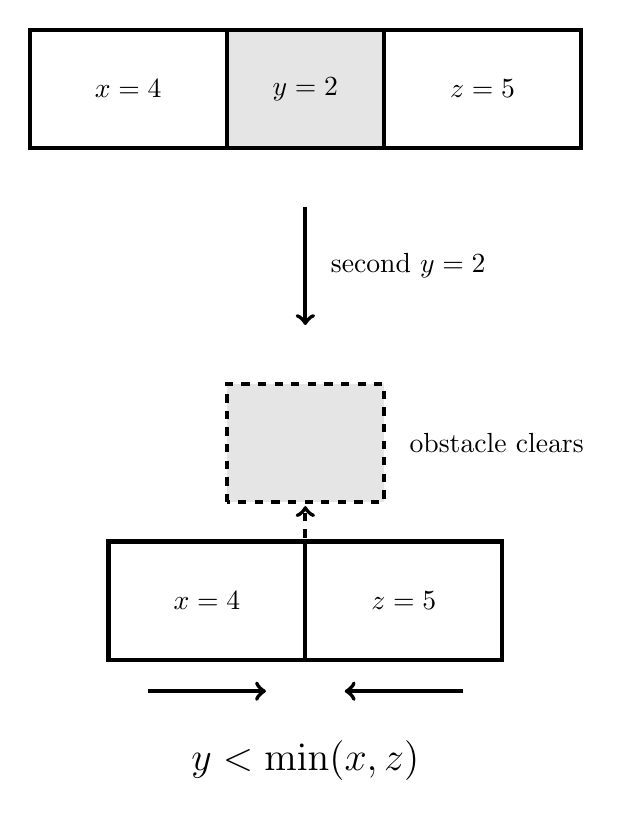
\begin{tikzpicture}

% 1. left-blue-block
\gid{left-blue-block}{
    \draw[line width=1.5pt] (-3.5, 5) rectangle (-1, 6.5);
}
% 2. left-lifetime-label
\gid{left-lifetime-label}{
    \node at (-2.25, 5.75) {$x=4$};
}

% 3. red-obstacle
\gid{red-obstacle}{
    \draw[line width=1.5pt, fill=black, fill opacity=0.1] (-1, 5) rectangle (1, 6.5);
}
% 4. obstacle-lifetime-label
\gid{obstacle-lifetime-label}{
    \node at (0, 5.75) {$y=2$};
}

% 5. right-blue-block
\gid{right-blue-block}{
    \draw[line width=1.5pt] (1, 5) rectangle (3.5, 6.5);
}
% 6. right-lifetime-label
\gid{right-lifetime-label}{
    \node at (2.25, 5.75) {$z=5$};
}

% 7. second-y-arrow
\gid{second-y-arrow}{
    \draw[->, line width=1.5pt] (0, 4.25) -- (0, 2.75);
    \node[right] at (0.2, 3.5) {second $y=2$};
}

% 8. vanishing-obstacle
\gid{vanishing-obstacle}{
    \draw[line width=1.5pt, dashed, fill=black, fill opacity=0.1] (-1, 0.5) rectangle (1, 2);
    \draw[->, line width=1.5pt, dashed] (0, 0.05) -- (0, 0.45);
}
% 9. obstacle-clears-label
\gid{obstacle-clears-label}{
    \node[right] at (1.2, 1.25) {obstacle clears};
}

% 10. meeting-blue-blocks
\gid{meeting-blue-blocks}{
    \draw[line width=1.5pt] (-2.5, -1.5) rectangle (0, 0);
    \node at (-1.25, -0.75) {$x=4$};
    \draw[->, line width=1.5pt] (-2, -1.9) -- (-0.5, -1.9);
    
    \draw[line width=1.5pt] (0, -1.5) rectangle (2.5, 0);
    \node at (1.25, -0.75) {$z=5$};
    \draw[->, line width=1.5pt] (2, -1.9) -- (0.5, -1.9);
}

% 11. fusion-condition
\gid{fusion-condition}{
    \node[below, font=\Large] at (0, -2.4) {$y < \min(x, z)$};
}

\end{tikzpicture}